\chapter{Introdução à Indexação}

\section{O que é indexação?}

Um índice, no contexto de \textit{dados estruturados}, é uma estrutura de dados que melhora a velocidade das operações de query de dados em uma tabela, ao custo de escritas adicionais e espaço de armazenamento para manter a estrutura do índice. Índices permitem localizar dados rapidamente sem precisar buscar sequencialmente em cada linha de uma tabela.

A maioria dos softwares de banco de dados inclui tecnologia de indexação que permite buscas em tempo sub-linear para melhorar o desempenho, já que a busca linear é ineficiente para grandes bancos de dados.

\cite{databaseindex:wiki}

\subsection{Busca por Semelhança}

No caso de \textit{dados não estruturados}, como bancos de dados multimídia e dados gerados por extração de características, a busca realizada não tem as mesmas características da busca exata. Ao invés disso, deseja-se encontrar os elementos mais semelhantes de um elemento de consulta.

Nesse tipo de cenário, o conceito de espaço métrico serve como modelo para o problema. Um espaço métrico é um conjunto $X$ com uma função de distância $d: X \times X \to \mathbb{R}$ que satisfaz as seguintes propriedades:

\begin{enumerate}
    \item $d(x, y) \geq 0$ (não-negatividade)
    \item $d(x, y) = 0 \iff x = y$ (identidade dos indiscerníveis)
    \item $d(x, y) = d(y, x)$ (simetria)
    \item $d(x, z) \leq d(x, y) + d(y, z)$ (desigualdade triangular)
\end{enumerate}

Um exemplo é o espaço euclidiano $\mathbb{R}^n$ com a norma $L^p$, tal que
$$d(x, y) = \left(\sum_{i = 1}^n|x_i - y_i|^p\right)^{1/p}$$
e para o caso $p = \infty$,
$$d(x, y) = \max_{1 \le i \le n}|x_i - y_i|$$

Diante disso, cada elemento do banco de dados é um elemento de $X$ e quanto menor a distância entre dois objetos, $d(x, y)$, maior a similaridade entre eles.

Note também que a busca por similaridade geralmente toma lugar em um espaço multidimensional (\cref{sec:multidimsearch}).

As buscas são de dois tipos

\textbf{Range Query} recupera todos os elementos até uma distância $r$ da query $q$, i.e.,
$$\{x \in X : d(x, q) \le r\}$$

\textbf{Nearest Neighbor Query} recupera os $k$ elementos mais próximos de $q$ em $X$, i.e., retornar $Y \subset X$ tal que $|Y| = k$ e $\forall y \in Y, \forall x \in X \setminus Y, d(y, q) \le d(x, q)$.

\subsubsection{Solução Força Bruta}

A maneira mais simples de fazer isso é realizando a comparação de todos os elementos do conjunto e retornar os $k$ mais próximos, com complexidade $O(n)$.

\begin{algorithm}
\caption{Busca por Força Bruta}
\label{alg:bruteforce}
\begin{algorithmic}[1]
\Procedure{BruteForceSearch}{$X, q, k$}
    \State $Y \gets \emptyset$
    \For{$x \in X$}
        \If{$|Y| < k$}
            \State $Y \gets Y \cup \{x\}$
        \Else
            \State $y \gets \arg\min_{y \in Y} d(y, q)$
            \If{$d(x, q) < d(y, q)$}
                \State $Y \gets Y \setminus \{y\} \cup \{x\}$
            \EndIf
        \EndIf
    \EndFor
    \State \Return $Y$
\EndProcedure
\end{algorithmic}
\end{algorithm}

No entanto, considerando o custo associado ao cálculo da distância, a escalabilidade linear é uma limitação para grandes conjuntos de dados.

Talvez com uso de GPU, paralelismo, seja possível melhorar o desempenho.

\section{Implementações de índices}

\subsection{B Tree}

Uma \textit{B-tree} é uma estrutura de dados em árvore auto-balanceada que mantém dados ordenados e permite buscas, acessos sequenciais, inserções e deleções em tempo logarítmico. A B-tree generaliza a árvore binária de busca, permitindo nós com mais de dois filhos.

É amplamente utilizada em sistemas de arquivos e bancos de dados. É uma estrutura que se beneficia da leitura e escrita em bloco, levando vantagem em um aspecto historicamente relevante, uma vez que o número de operações de I/O (em discos magnéticos) era igualmente relevante para o desempenho quanto o número de operações de comparação.

Foi inventada por Rudolf Bayer e Edward M. McCreight em 1972 \cite{btree:bayer1970} (o B não foi explicado por eles).

% Quote
\begin{quotation}
    \it What Rudy (Bayer) likes to say is, the more you think about what the B in B-Tree means, the better you understand B-Trees!
\end{quotation}

Os principais algoritmos associados a B-trees são: busca (\cref{alg:btree_search}) e inserção (\cref{alg:btree_insertion}) (existem variações para a operação de deleção).

São necessárias duas funções auxiliares para a inserção: \textsc{splitChild}, que divide um nó cheio em dois, e \textsc{insertNonFull}, que insere uma chave em um nó não cheio.

\textit{Bulk loading?}

\begin{algorithm}
\caption{Algoritmo de busca na B Tree, assumindo que a chave $k$ é o valor a ser buscado e $x$ é o nó onde a busca começa.}
\label{alg:btree_search}
\begin{algorithmic}[1]
\Procedure{BtreeSearch}{$x, k$}
    \State $i \gets 0$
    \While{$i < x.n$ \textbf{and} $k > x.key[i]$}
        \State $i \gets i + 1$
    \EndWhile
    \If{$i < x.n$ \textbf{and} $k = x.key[i]$}
        \State \Return $x$
    \EndIf
    \If{$x.leaf$}
        \State \Return \textbf{None}
    \EndIf
    \State \Return \Call{BtreeSearch}{$x.child[i], k$}
\EndProcedure
\end{algorithmic}
\end{algorithm}

\begin{algorithm}
\caption{Algoritmo de inserção na B Tree, assumindo que a chave $k$ é o valor a ser inserido.}
\label{alg:btree_insertion}
\begin{algorithmic}[1]
\Procedure{BtreeInsert}{$T, k$}
    \State $r \gets T.root$
    \If{$r.n = 2(T.d) - 1$}
        \State $s \gets$ \textbf{new} Node
        \State $T.root \gets s$
        \State $s.child[1] \gets r$
        \State \Call{splitChild}{$s, 1$}
        \State \Call{insertNonFull}{$s, k$}
    \Else
        \State \Call{insertNonFull}{$r, k$}
    \EndIf
\EndProcedure
\end{algorithmic}
\end{algorithm}

\cite{btree:wiki,btree:comer1979,btree:bayer1970}

\subsection{B+ Tree}

Uma B+ tree pode ser vista como uma B-tree onde cada nó contém apenas chaves (não pares chave-valor), com um nível adicional de folhas ligadas na parte inferior.

O principal valor de uma B+ tree está no armazenamento de dados para recuperação eficiente em um contexto de armazenamento orientado a blocos, como sistemas de arquivos. Diferente das árvores binárias de busca, as B+ trees têm um fanout muito alto (número de ponteiros para nós filhos em um nó, tipicamente na ordem de 100 ou mais), o que reduz o número de operações de I/O necessárias para encontrar um elemento na árvore.

Aplicações: iDistance

\cite{bptree:wiki}

\section{Indexação Multidimensional}
\label{sec:multidimsearch}

Exemplo de como estava sendo realizada a indexação multidimensional em multimidia(imagens)

Efficient and Effective Querying by Image Content

\subsection{R-Tree}

Usada para multidimensional

\subsection{KD-Tree}

1975 \cite{kdtree:wiki,kdtree:bentley1975}

$O(\log n)$ em dimensões 2 e 3.

\begin{figure}
    \centering
    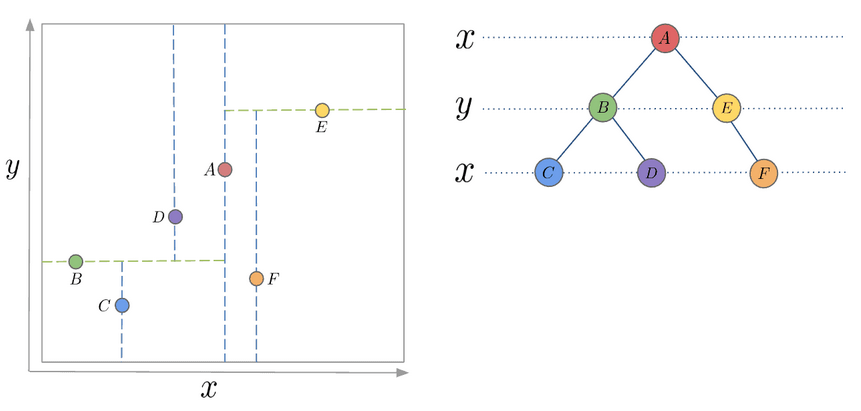
\includegraphics[width=0.5\textwidth]{imgs/kdtree.png}
    \caption{Exemplo de uma KD-Tree.}
    \label{fig:kdtree}
\end{figure}

\subsection{M-Tree}

Usada para espaços métricos

\cite{mtree:ciaccia1997}

\subsection{}

Survey \cite{multidimensionalmethods:gaede1998}

\section{The Curse of Dimensionality}

O termo ``\textit{curse of dimensionality}'' é atribuído a Richard Bellman, que se referiu isso no contexto de programação dinâmica e o impacto do número de estados na performance do algoritmo. É o fenômeno relacionado ao aumento da dificuldade/complexidade de uma tarefa com o aumento da dimensionalidade dos dados. Isso significa que a tarefa pode ser realizada de forma satisfatória em dimensões baixas, mas tem performance muito pior ou se torna inviável em dimensões altas. Existem outras definições, como uma associada ao ``\textit{fenômeno de Hughes}'' \cite{meanacc:hughes1968}, mas em geral o termo é utilizado para descrever dificuldades encontradas ao entrar em um contexto com alta dimensionalidade. 

\subsection{Conceito de Dimensão}

Dimensão intrínseca

\subsection{Impacto na Busca por Similaridade}

O conceito de dimensão está associado, em problemas de busca por similaridade, a dificuldade da busca.

Pensando na distribuição de pontos, é possível fazer uma pequena análise que demonstre a esparsidade dos dados em altas dimensões. Para isso, calcularemos a razão de volumes em uma esfera inscrita em um cubo. A princípio, a razão entre os volumes é de
$$\left(\frac{4}{3} \pi r^3\right)\frac{1}{8r^3} \approx 0.52$$
conforme a dimensão $d$ aumenta, a razão 
$$\left(\frac{2r^d\pi^{d/2}}{d\Gamma(d/2)}\right)\frac{1}{(2r)^d} \to 0$$
indicando que o volume da hiperesfera se torna insignificante em relação ao volume do hipercubo. \cite{cursedim:wiki}

Em particular, no contexto de espaços métricos, as medidas de distância entre pares de pontos colapsam, fazendo com que a distância entre todos os pontos seja aproximadamente a mesma. Dessa maneira, descartar elementos com uma distância maior que a média, em um cenário com alta dimensionalidade, descarta poucos elementos.

\begin{figure}
    \centering
    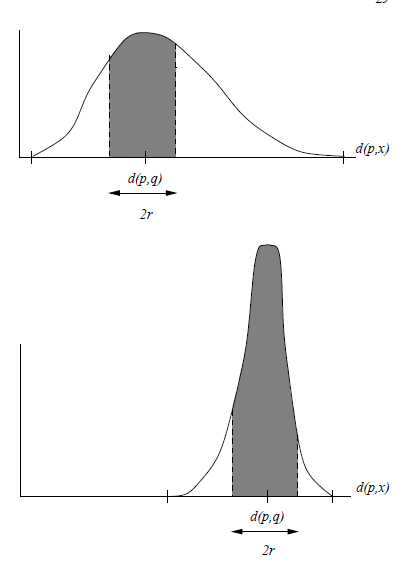
\includegraphics[width=0.5\textwidth]{imgs/distribution_curse.png}
    \caption{Ilustração da ``\textit{curse of dimensionality}'' na distribuição de distâncias.}
    \label{fig:distribution_curse}
\end{figure}


Na kd-tree, a complexidade é
$O(d N^{1 - 1/k})$\cite{worstcase:lee1977}.


\cite{searching:navarro2002,searching:chavez2001}

\subsection{}

\printbibliography